\chapter{Introduction}

Accelerators are becoming more important in \acrfull{hpc} to increase computing power. Accelerators have compute units specialized for a single domain. \acrshortpl{gpu} are by far the most common type of accelerator, exploiting data level parallelism to achieve high throughput for highly parallelizable workloads. \acrshortpl{gpu} are used for graphics operations, but also for other more compute focused workloads.
Due to the prevalence of \acrshortpl{gpu}, \acrshort{gpu} research is becoming more essential.

% \textcolor{red}{This is a part of enabling GPU research at in CAL at NTNU.}

\Gls{vortex} is an open-source \acrshort{gpgpu} with a focus on enabling architecture research. In this thesis I continue the work done in my project thesis \cite{Aurud_Project} and the master's thesis of M. Rekdal \cite{Rekdal_Master}. In my project thesis\cite{Aurud_Project}, I investigated the performance of \Gls{vortex}, in addition to implementing \acrfull{csv} breaking down the cycles. In the project I found that \Gls{vortex} is mainly stalling due to instructions waiting for memory requests to resolve, making it latency bound. This was possibly due to issues with the schedulers and frontend of \Gls{vortex}' pipeline. The issue scheduler is at times unable to issue ready instructions reducing its throughput and ability to exploit parallelism. Additionally I observed that the frontend of \Gls{vortex}' pipeline is struggling to fetch enough instructions to enable the \acrshort{gpu} to hide stalls.

In this thesis first I describe in detail the issues found in my project before I propose and implement solutions for them. To obtain more and better results, I also implement most of the Rodinia benchmarks to run on \Gls{vortex}.  

\textcolor{red}{Describe why FPGA simulation is great and why this is a motivation for using vortex. A common method for evaluating computer architecture is software simulation. This is troublesome for larger systems as it is slow}

\textcolor{red}{While Vortex allows for FPGA simulation, it has a main issue, memory bandwidth and latency scaled to the throughput of the GPU. While work is being done at CAL to solve this, I have to continue using software simulation. }

\textcolor{red}{This work is also about getting to know Vortex and its architecture. Improving the Vortex environment with benchmarks and tools (\acrshort{csv}) which can be used on FPGAs}

\section{Assignment Interpretation}

In this thesis I will continue the work done in my project thesis\cite{Aurud_Project}. The overarching goal of the my project- and master thesis is to aid the \acrfull{cal} at NTNU to simulate and evaluate \acrshort{gpu}s using \acrshort{fpga}s. I define the following list of tasks based on my interpretation of \hyperref[chap:assignment]{the assignment text}:

\begin{itemize}
    \item[\textbf{T1}] Propose and implement a set of improvements to the \Gls{vortex} \acrshort{gpu} based on results and \acrshort{cpi} stacks obtained in the project thesis.
    \item[\textbf{T2}] Improve \acrshort{csv} to give a better overview of the issue stage. 
    \item[\textbf{T3}] Evaluate the implemented improvements.
    \item[\textbf{T4}] If time permits, evaluate the observed problems and proposed solutions using a commonly used GPU benchmarks suite such as Rodinia.
\end{itemize}

Task \textbf{T2} was added during development of the improvements, as I discovered that my existing version of \acrshort{csv} was too connected to \Gls{vortex}' issue scheduler. This blocked \acrshort{csv} from giving a good overview of the issue stage and stall causes.

\section{Contributions}

In this thesis I make the following key contributions:
\begin{itemize}
    \item[\textbf{C1}] I propose and implement changes to \Gls{vortex}' fetch, decode and issue stage to increase fetch and issue bandwidth, solving the problems identified in my project thesis.
    \item[\textbf{C2}] I improve upon \acrshort{csv}, enabling it to identify the stall cause for all warps in the instruction buffer and attributing them accordingly.
    \item[\textbf{C3}] I evaluate the implemented improvements using \acrshort{cpi} stacks and other collected performance metrics. I find that the changes are able to move the frontend bottleneck to the backend of the \Gls{gpu}, showing that \Gls{vortex} is unable to hide latency stalls.
    \item[\textbf{C4}] I expand \Gls{vortex}' benchmark suite to include most of the \Gls{rodinia} benchmarks. I additionally improve core components of \Gls{vortex}' mechanisms to collect performance metrics, making it more accurate and allowing multi-kernel programs to be used for benchmarking.  
\end{itemize}

Figure \ref{fig:task-contribution} describes how the tasks and contributions relate and where in the project the contributions are made.

\begin{figure}
    \centering
    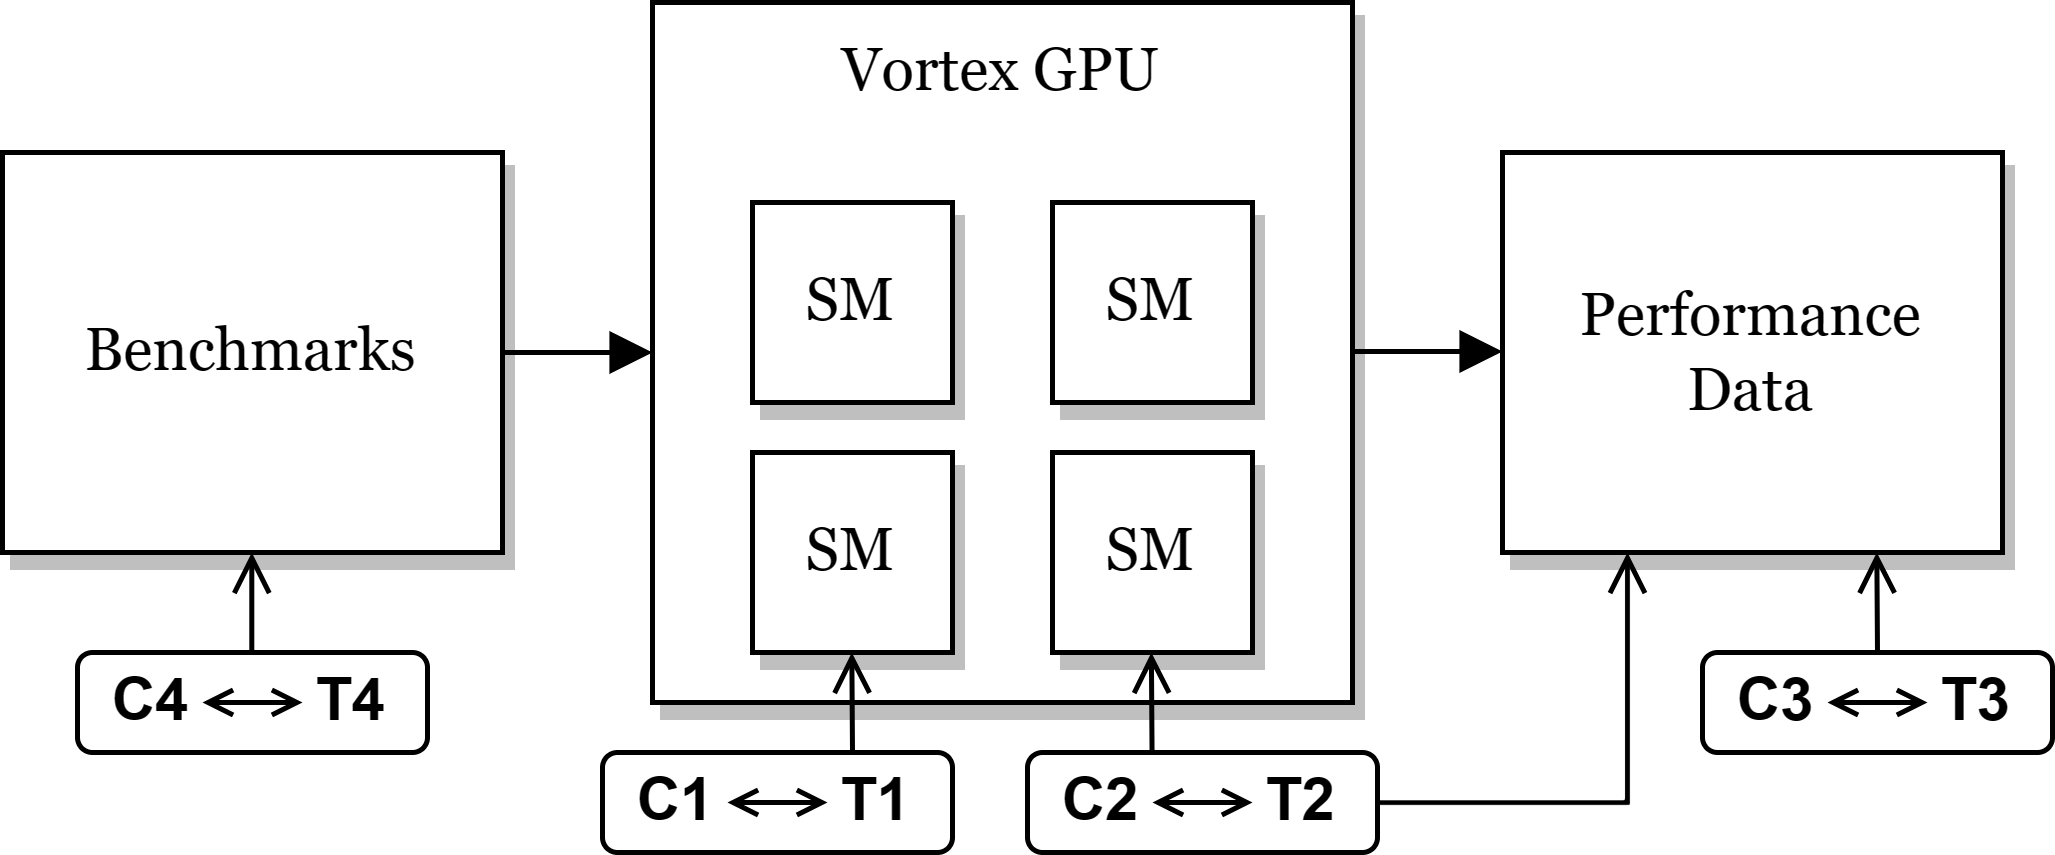
\includegraphics[width=\textwidth]{figures/task-contribution-2.png}
    \caption[Relating tasks and contributions to the project.]{Illustration of how the tasks and contributions relate and where in the project the contributions are made.}
    \label{fig:task-contribution}
\end{figure}

\section{Outline}

Following is the outline for the rest of the thesis:

\begin{itemize}
    \item \textbf{Chapter 2} covers background information regarding GPUs, GPU simulation, stall inspection and the architecture of \Gls{vortex}.
    \item \textbf{Chapter 3} details all of the changes/improvements I have done to the Vortex architecture.
    \item \textbf{Chapter 4} contains details regarding how Rodinia benchmarks were altered to run on \Gls{vortex}.
    \item \textbf{Chapter 5} describes my methodology for collecting performance metrics and generating \acrlong{csv}.
    \item \textbf{Chapter 6} includes information regarding the experimental setup and \Gls{vortex} configuration.
    \item \textbf{Chapter 7} contains the results and analysis. Additionally, I present a sensitivity analysis.
    \item \textbf{Chapter 8} contains the conclusion in addition to ideas for further work.
\end{itemize}

\begin{figure}
    \centering
    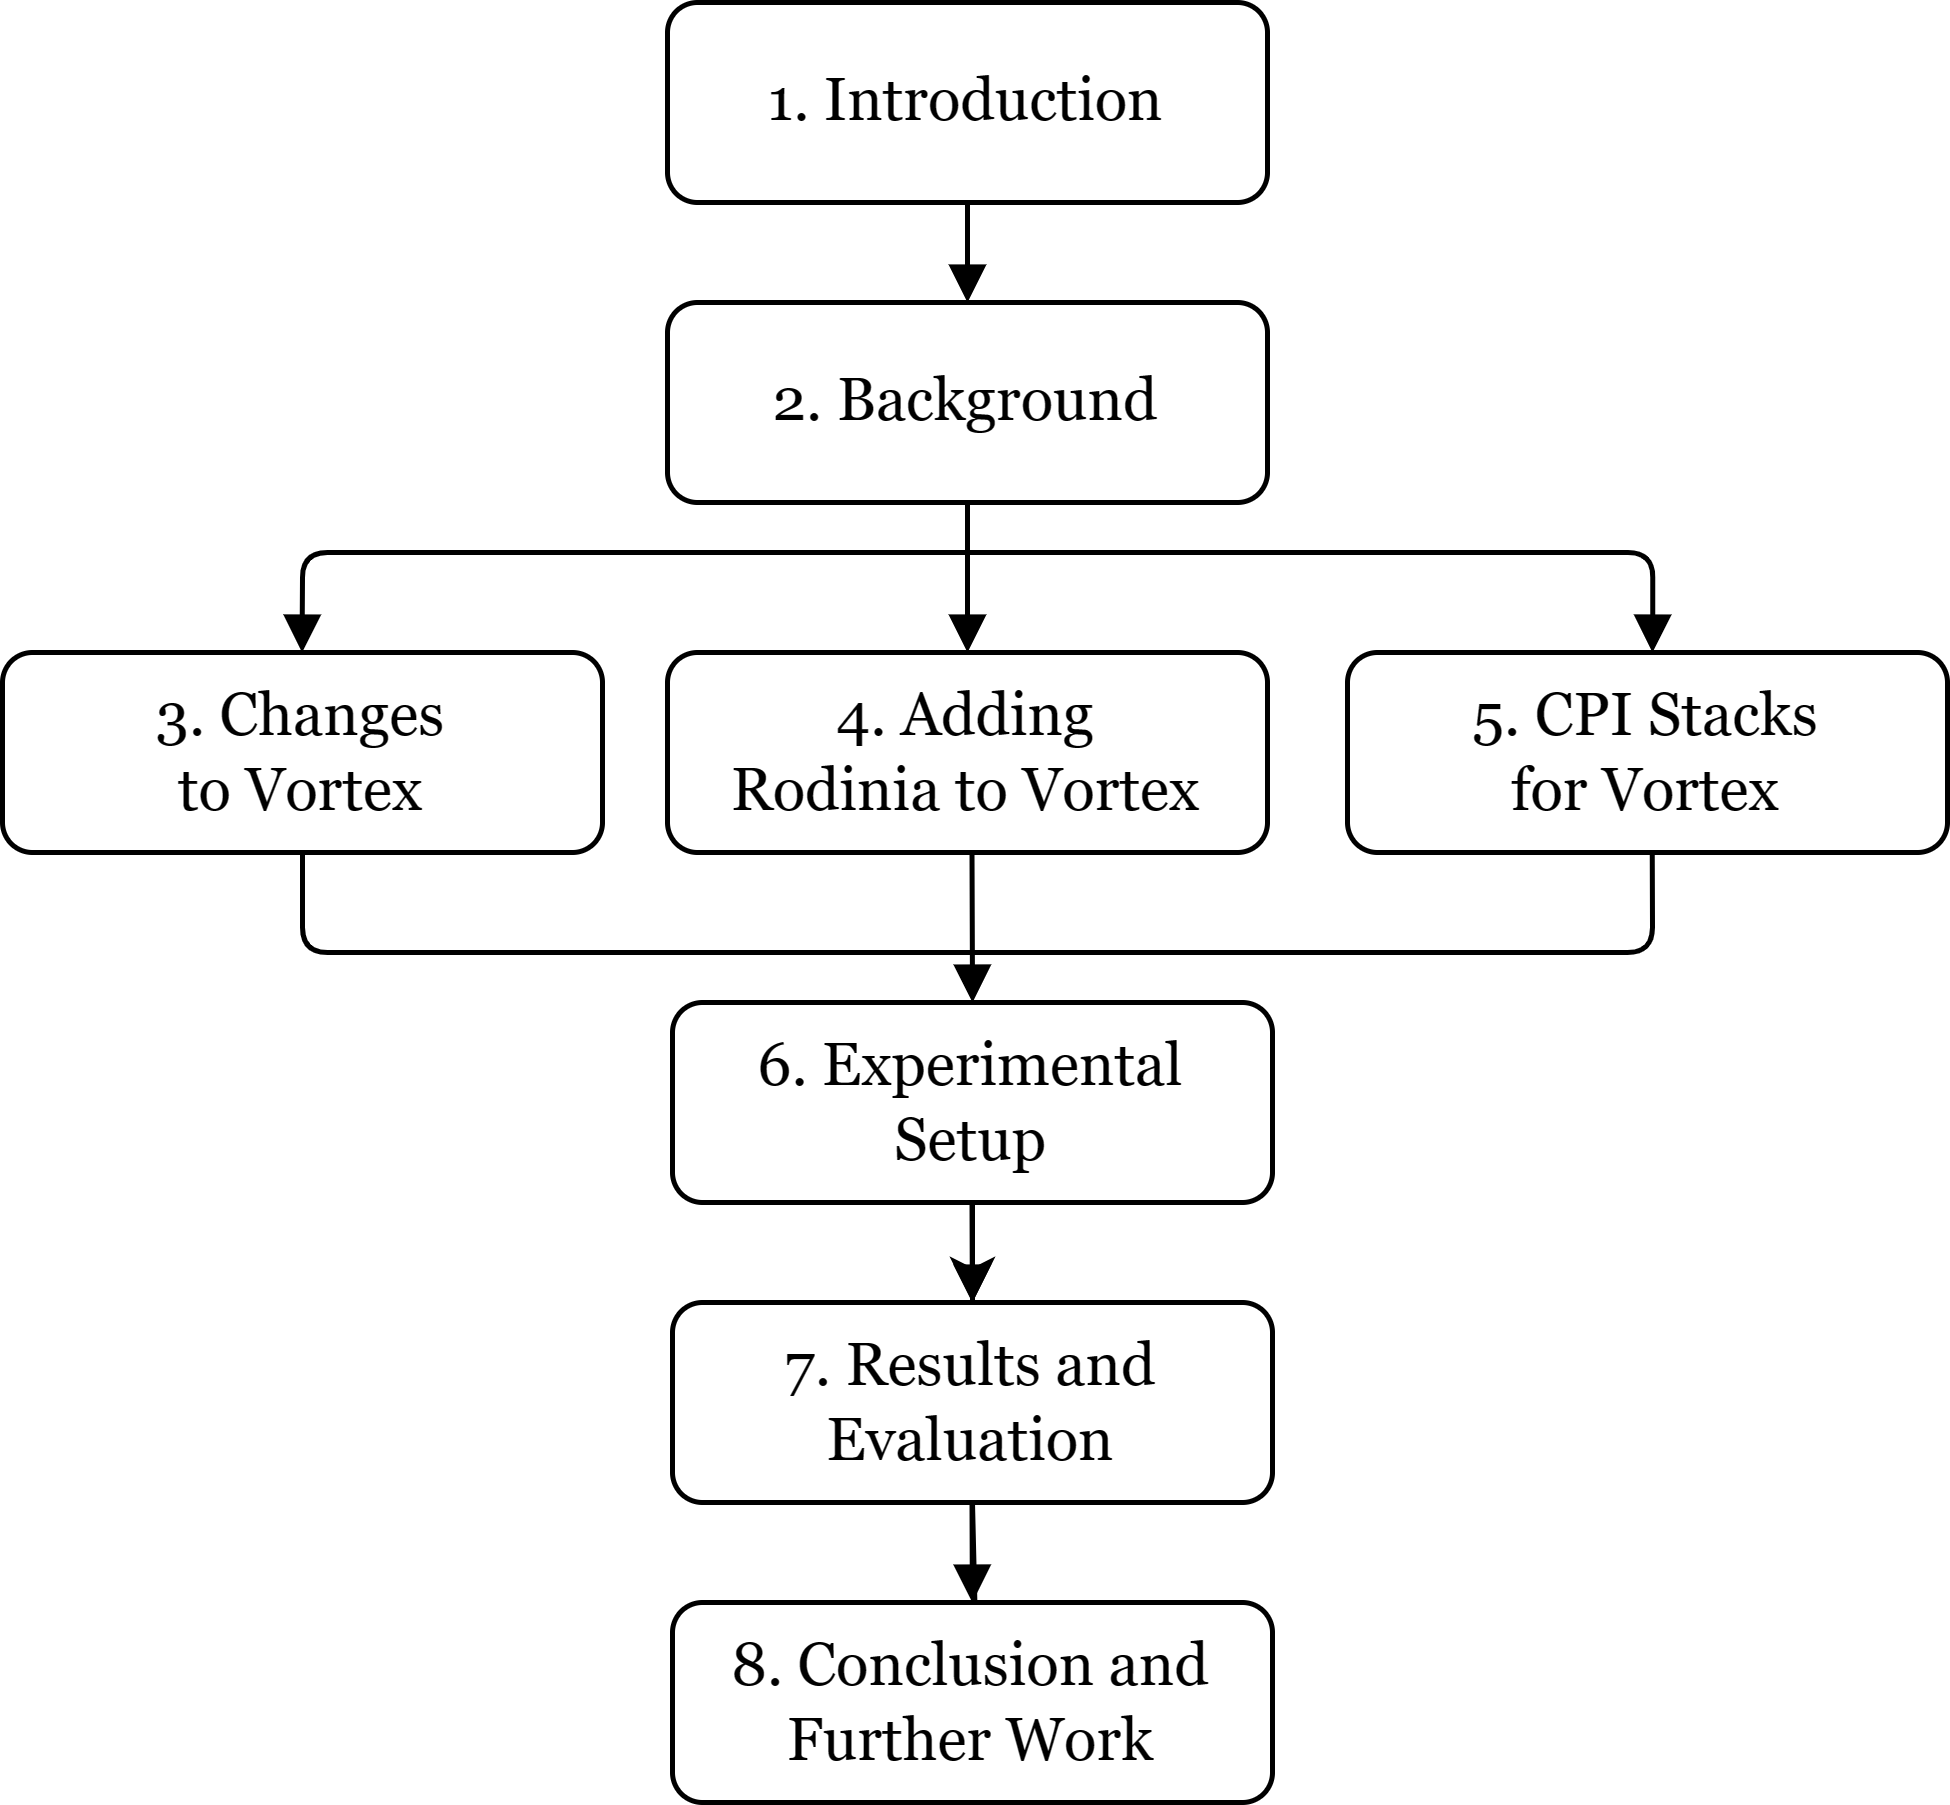
\includegraphics[width=0.8\textwidth]{figures/thesis-outline.png}
    \caption[Outline of the thesis]{Outline of chapters in the thesis. Chapter 3, 4 and 5 cover the contributions made by me.}
    \label{fig:thesis_outline}
\end{figure}


